%% SPDX-FileCopyrightText: 2026 Jeremy Martinon
%% SPDX-License-Identifier: GPL-3.0-or-later
%% Adapted from the author-supplied TNTex.tex for the documentation.
\documentclass[10pt,border=6pt]{standalone}
\usepackage{pgfplots}
\usepackage{xcolor}
\pgfplotsset{compat=1.15}
\usepackage{mathrsfs}
\usetikzlibrary{arrows}
\pagestyle{empty}

\definecolor{greenBox}{RGB}{224,255,223}
\definecolor{blueBox}{RGB}{239,239,254}
\colorlet{green_6j}{green!15}
\colorlet{blue_booster}{blue!15}
% Keep labels dark on the opaque pastel tensors in both website themes.
\definecolor{tensorLabel}{HTML}{1A1A1A}

\newcommand{\radius}{0.75cm} % define a radius constant
\newcommand{\radiusP}{0.35cm}
\tikzset{every node/.style={font=\LARGE}}

\begin{document}
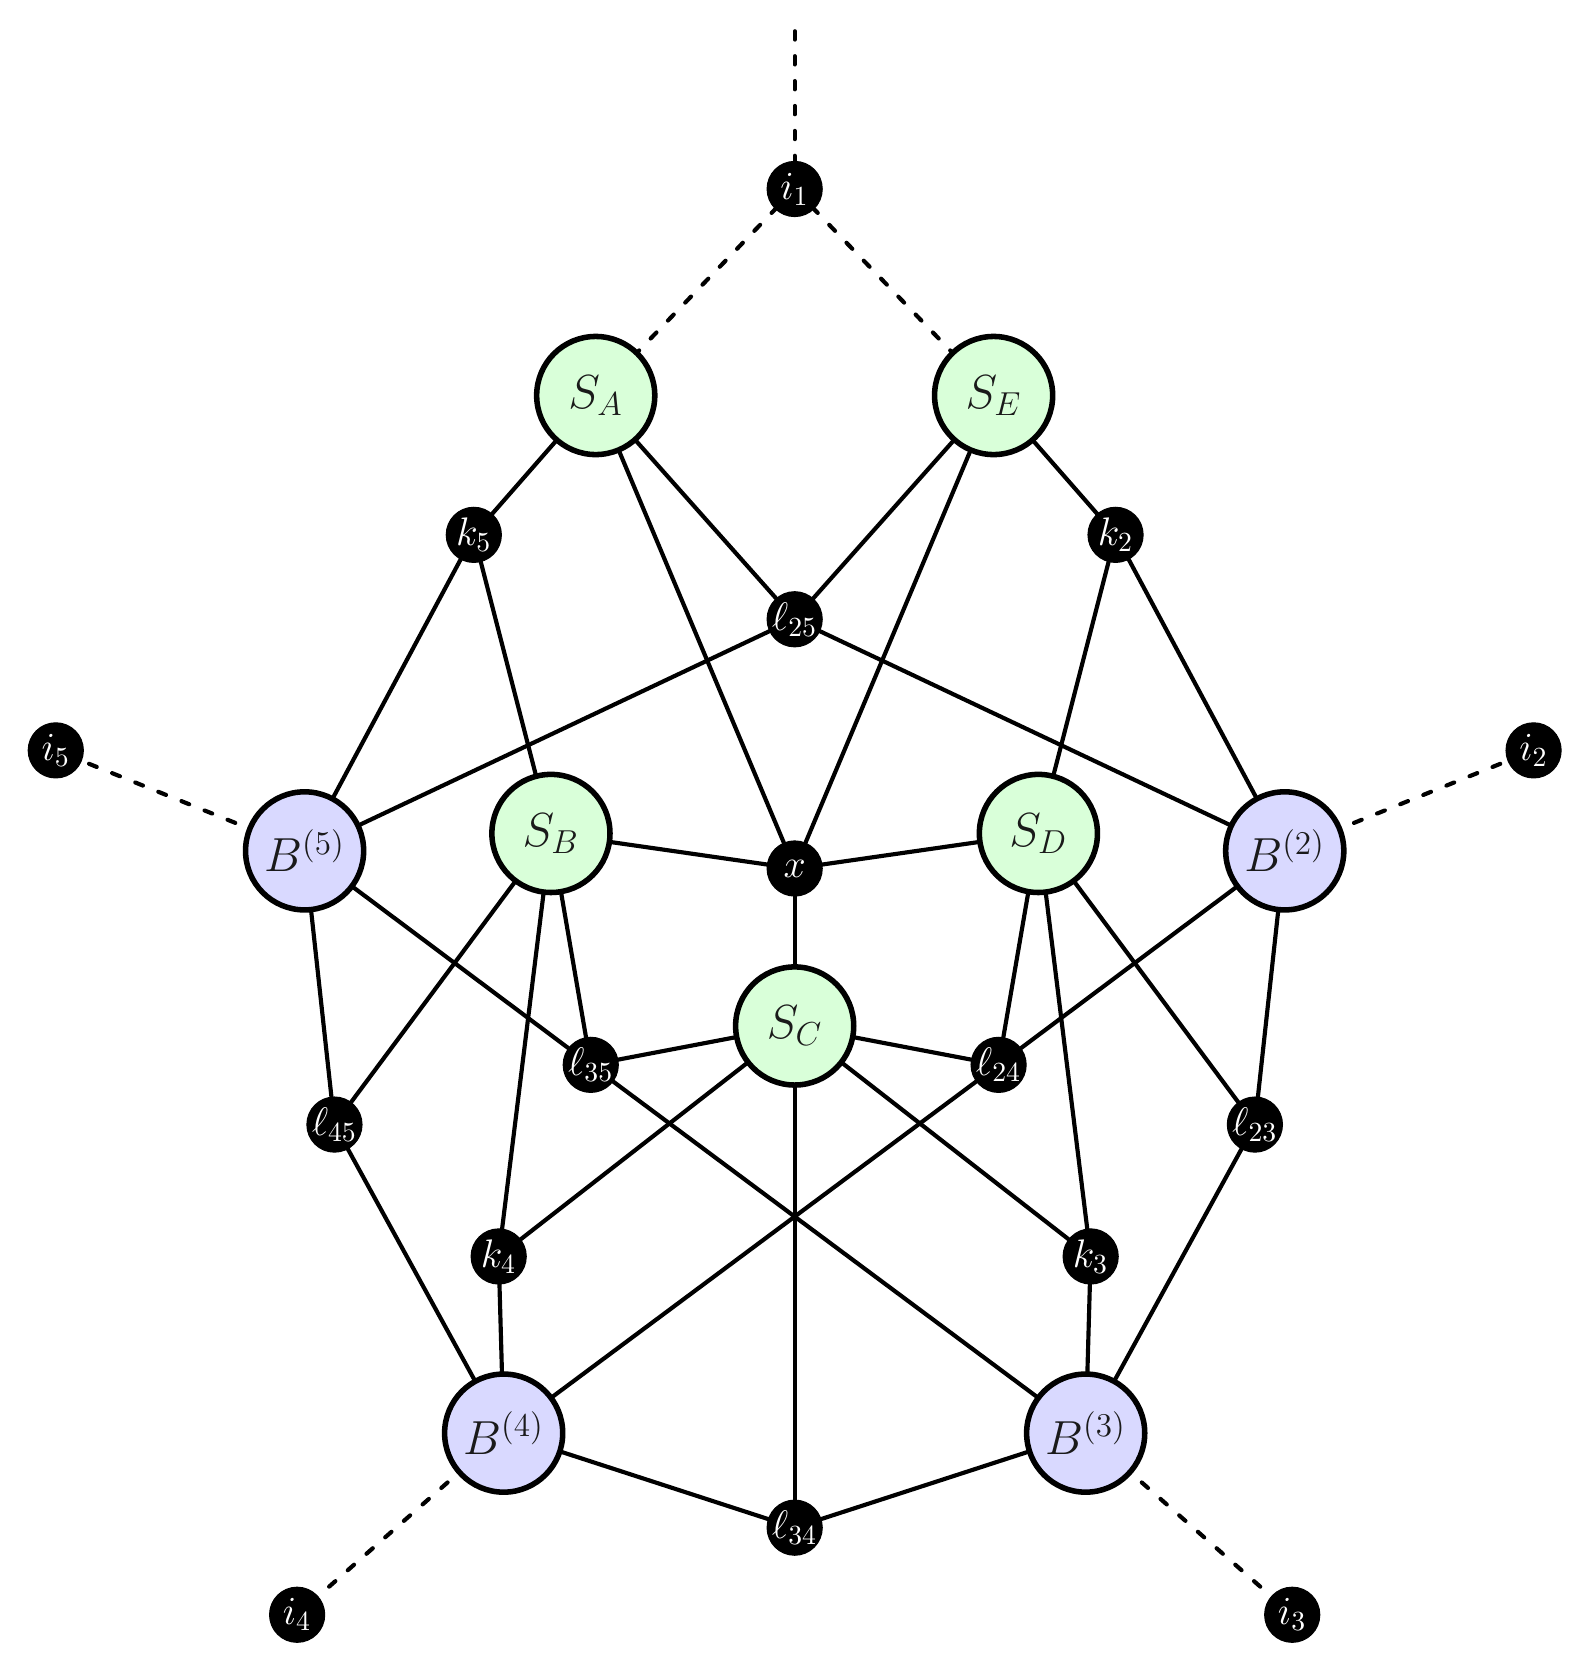
\begin{tikzpicture}[line cap=round,line join=round,>=triangle 45,x=1cm,y=1cm]

\draw [line width=1.5pt,loosely dashed] (0,12.629649993391295)-- (2.5266029505691034,10.006789035139859);

\draw [line width=1.5pt] (2.5266029505691034,10.006789035139859)-- (4.075038937970557,8.237147906681058);
\draw [line width=1.5pt,loosely dashed] (6.223888879670533,4.223854633211988)-- (9.38396232334697,5.5);
\draw [line width=1.5pt] (4.075038937970557,8.237147906681058)-- (6.223888879670533,4.223854633211988);
\draw [line width=1.5pt] (0,7.165022346906796)-- (2.5266029505691034,10.006789035139859);
\draw [line width=1.5pt] (0,4)-- (2.5266029505691034,10.006789035139859);
\draw [line width=1.5pt] (0,7.165022346906796)-- (6.223888879670533,4.223854633211988);
\draw [line width=1.5pt] (4.075038937970557,8.237147906681058)-- (3.095416170430862,4.445059774269338);
\draw [line width=1.5pt] (6.223888879670533,4.223854633211988)-- (5.844680066429361,0.747773845167912);
\draw [line width=1.5pt] (6.223888879670533,4.223854633211988)-- (2.589804419442632,1.5061914716502558);
\draw [line width=1.5pt] (3.095416170430862,4.445059774269338)-- (2.589804419442632,1.5061914716502558);
\draw [line width=1.5pt] (2.589804419442632,1.5061914716502558)-- (0,2);
\draw [line width=1.5pt] (0,2)-- (3.7590315936029133,-0.9270650799805972);
\draw [line width=1.5pt] (3.7590315936029133,-0.9270650799805972)-- (3.095416170430862,4.445059774269338);
\draw [line width=1.5pt] (3.095416170430862,4.445059774269338)-- (5.844680066429361,0.747773845167912);
\draw [line width=1.5pt,loosely dashed] (3.6958301247293845,-3.1707172249908644)-- (6.318691082980827,-5.47757083887466);
\draw [line width=1.5pt] (0,-4.371545133587909)-- (3.6958301247293845,-3.1707172249908644);
\draw [line width=1.5pt] (0,-4.371545133587909)-- (0,2);
\draw [line width=1.5pt] (3.7590315936029133,-0.9270650799805972)-- (3.6958301247293845,-3.1707172249908644);
\draw [line width=1.5pt] (5.844680066429361,0.747773845167912)-- (3.6958301247293845,-3.1707172249908644);
\draw [line width=1.5pt] (0,4)-- (3.095416170430862,4.445059774269338);
\draw [line width=1.5pt,loosely dashed] (0,12.629649993391295)-- (-2.526602950569102,10.006789035139859);
\draw [line width=1.5pt] (0,7.165022346906796)-- (-2.526602950569102,10.006789035139859);
\draw [line width=1.5pt] (0,4)-- (-2.526602950569102,10.006789035139859);
\draw [line width=1.5pt] (-2.526602950569102,10.006789035139859)-- (-4.0750389379705565,8.237147906681058);
\draw [line width=1.5pt] (-4.0750389379705565,8.237147906681058)-- (-3.0954161704308616,4.445059774269338);
\draw [line width=1.5pt] (-4.0750389379705565,8.237147906681058)-- (-6.2238888796705325,4.223854633211989);
\draw [line width=1.5pt,loosely dashed] (-6.2238888796705325,4.223854633211989)-- (-9.38396232334697,5.5);
\draw [line width=1.5pt] (-6.2238888796705325,4.223854633211989)-- (-5.844680066429361,0.7477738451679127);
\draw [line width=1.5pt] (-3.0954161704308616,4.445059774269338)-- (-5.844680066429361,0.7477738451679127);
\draw [line width=1.5pt] (-6.2238888796705325,4.223854633211989)-- (-2.589804419442632,1.506191471650256);
\draw [line width=1.5pt] (-3.0954161704308616,4.445059774269338)-- (-2.589804419442632,1.506191471650256);
\draw [line width=1.5pt] (-2.589804419442632,1.506191471650256)-- (0,2);
\draw [line width=1.5pt] (0,2)-- (-3.7590315936029133,-0.9270650799805967);
\draw [line width=1.5pt] (-3.7590315936029133,-0.9270650799805967)-- (-3.695830124729385,-3.170717224990864);
\draw [line width=1.5pt] (0,-4.371545133587909)-- (-3.695830124729385,-3.170717224990864);
\draw [line width=1.5pt,loosely dashed] (-3.695830124729385,-3.170717224990864)-- (-6.318691082980828,-5.477570838874659);
\draw [line width=1.5pt] (-5.844680066429361,0.7477738451679127)-- (-3.695830124729385,-3.170717224990864);
\draw [line width=1.5pt] (0,4)-- (0,2);
\draw [line width=1.5pt] (0,4)-- (-3.0954161704308616,4.445059774269338);
\draw [line width=1.5pt] (0,7.165022346906796)-- (-6.2238888796705325,4.223854633211989);
\draw [line width=1.5pt] (-3.7590315936029133,-0.9270650799805976)-- (-3.0954161704308625,4.445059774269338);
\draw [line width=1.5pt] (3.6958301247293845,-3.1707172249908644)-- (-2.589804419442632,1.506191471650256);
\draw [line width=1.5pt] (-3.695830124729385,-3.170717224990864)-- (2.589804419442632,1.5061914716502558);
\draw [line width=1.5pt,loosely dashed] (0,12.629649993391295)-- (0,14.652096997344211);

\draw [fill=black] (0,12.629649993391295) circle (\radiusP)node{\Large\textcolor{white}{$i_1$}};
\draw [fill=black] (0,7.165022346906796) circle (\radiusP)node{\Large\textcolor{white}{$\ell_{25}$}};

\draw [fill=black] (0,4) circle (\radiusP)node{\Large\textcolor{white}{$x$}};

\draw [fill=black] (0,-4.371545133587909) circle(\radiusP)node{\Large\textcolor{white}{$\ell_{34}$}};

\draw [fill=black] (2.589804419442632,1.5061914716502558) circle (\radiusP)node{\Large\textcolor{white}{$\ell_{24}$}};
\draw [fill=black] (3.7590315936029133,-0.9270650799805972) circle (\radiusP)node{\Large\textcolor{white}{$k_3$}};

\draw [fill=black] (4.075038937970557,8.237147906681058) circle(\radiusP)node{\Large\textcolor{white}{$k_2$}};

%\draw [fill=black] (9.38396232334697,4.19225389877522) circle (\radiusP)node{\Large\textcolor{white}{$i_2$}};
\draw [fill=black] (9.38396232334697,5.5) circle (\radiusP)node{\Large\textcolor{white}{$i_2$}};

\draw [fill=black] (5.844680066429361,0.747773845167912) circle (\radiusP)node{\Large\textcolor{white}{$\ell_{23}$}};

\draw [fill=black] (6.318691082980827,-5.47757083887466) circle (\radiusP)node{\Large\textcolor{white}{$i_3$}};
\draw [fill=black] (-4.0750389379705565,8.237147906681058) circle (\radiusP)node{\Large\textcolor{white}{$k_5$}};
\draw [fill=black] (-9.38396232334697,5.5) circle (\radiusP)node{\Large\textcolor{white}{$i_5$}};
\draw [fill=black] (-5.844680066429361,0.7477738451679127) circle (\radiusP)node{\Large\textcolor{white}{$\ell_{45}$}};
\draw [fill=black] (-2.589804419442632,1.506191471650256) circle (\radiusP)node{\Large\textcolor{white}{$\ell_{35}$}};

\draw [fill=black] (-3.7590315936029133,-0.9270650799805967) circle (\radiusP)node{\Large\textcolor{white}{$k_4$}};
\draw [fill=black] (-6.318691082980828,-5.477570838874659) circle (\radiusP)node{\Large\textcolor{white}{$i_4$}};
%\draw [line width=2pt, fill=black,opacity=1] (2,10) circle (\radius) node{\textcolor{white}{$\ell$}};

\draw [line width=2pt,fill=green_6j,opacity=1] (2.5266029505691034,10.006789035139859) circle (\radius)node[text=tensorLabel]{$S_E$};

\draw [line width=2pt,fill=blue_booster,opacity=1] (6.223888879670533,4.223854633211988) circle (\radius)node[text=tensorLabel]{$B^{(2)}$};

\draw [line width=2pt,fill=green_6j,opacity=1] (3.095416170430862,4.445059774269338) circle (\radius)node[text=tensorLabel]{$S_D$};

\draw [line width=2pt,fill=green_6j,opacity=1] (0,2) circle (\radius)node[text=tensorLabel]{$S_C$};

\draw [line width=2pt,fill=blue_booster,opacity=1] (3.6958301247293845,-3.1707172249908644) circle (\radius)node[text=tensorLabel]{$B^{(3)}$};

\draw [line width=2pt,fill=green_6j,opacity=1] (-2.526602950569102,10.006789035139859) circle (\radius)node[text=tensorLabel]{$S_A$};

\draw [line width=2pt,fill=green_6j,opacity=1] (-3.0954161704308616,4.445059774269338) circle (\radius)node[text=tensorLabel]{$S_B$};

\draw [line width=2pt,fill=blue_booster,opacity=1] (-6.2238888796705325,4.223854633211989) circle (\radius)node[text=tensorLabel]{$B^{(5)}$};

\draw [line width=2pt,fill=blue_booster,opacity=1] (-3.695830124729385,-3.170717224990864) circle (\radius)node[text=tensorLabel]{$B^{(4)}$};

\end{tikzpicture}
\end{document}
